% !TeX program = lualatex
% このファイルは LuaLaTeX で処理してください(pdfLaTeX/upLaTeXでは動作しません)。
\documentclass[a4paper,11pt]{ltjsarticle}

\usepackage{amsmath,amssymb,mathtools}
\usepackage{siunitx}
\usepackage{geometry}
\geometry{a4paper,top=15mm,bottom=18mm,left=14mm,right=14mm}
\usepackage{tikz}
\usetikzlibrary{arrows.meta,positioning,calc}
\usepackage[most]{tcolorbox}
\usepackage{booktabs}
\usepackage{array}
\usepackage{multirow}
\usepackage{enumitem}

\setlength{\parindent}{0pt}
\setlength{\parskip}{2pt}
\renewcommand{\arraystretch}{2.6}

\newcommand{\banner}[1]{%
  \begin{tcolorbox}[colback=black,coltext=white,boxrule=0pt,sharp corners,
    left=8pt,right=8pt,top=5pt,bottom=5pt,before skip=8pt,after skip=8pt]
    {\Large\bfseries #1}
  \end{tcolorbox}}

\newtcolorbox{pointbox}[1][]{%
  colback=black!4,colframe=black,boxrule=0.6pt,arc=1mm,
  left=6pt,right=6pt,top=4pt,bottom=4pt,#1}

\pagestyle{plain}

\begin{document}

\banner{弦の振動}

下の図は，長さ $L$ の弦に生じる定在波のようすを表している(固定端の位置に破線，弦の中央付近に見える点線は，節または腹の位置の目安として引いてある)。それぞれの図をよく見て，表の空欄をうめよ。弦を伝わる波の速さを $v$ とする。

\begin{center}
\begin{tabular}{c|c|c|>{\centering\arraybackslash}p{2.6cm}|>{\centering\arraybackslash}p{3.0cm}|c|>{\centering\arraybackslash}p{1.5cm}|}
\cline{2-7} % 表部分（2〜7列目）の上側の罫線。弦の図の列には引かない

% ---- ヘッダー行 ----
\makebox[3.6cm][l]{\hspace{-1.2cm}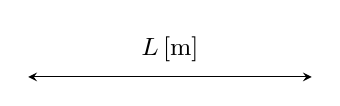
\begin{tikzpicture}[x=1cm,y=1cm]
  \draw[<->,>=stealth] (0,0) -- (3.6,0); % 弦全体の長さ L を示す両矢印
  \node[font=\small] at (1.8,0.35) {$L\,[\mathrm{m}]$}; % 矢印の上に長さのラベルを表示
\end{tikzpicture}}
& \textbf{腹}
& \textbf{振動の種類}
& \textbf{波長 $\lambda\,[\mathrm{m}]$}
& \textbf{振動数 $f\,[\mathrm{Hz}]$}
& \textbf{音の高さ}
& \textbf{例} \\
\cline{2-7} % ヘッダー行の下側の罫線（弦の図の列には引かない）

% ---- 基本振動 (n=1) ----
\makebox[3.6cm][l]{\hspace{-1.2cm}\begin{tikzpicture}[x=0.6cm,y=0.6cm]
  \draw[dashed] (0,2.1) -- (0,-2.1); % 左端（固定端）にある節の位置を示す点線
  \draw[dashed] (6,2.1) -- (6,-2.1); % 右端（固定端）にある節の位置を示す点線
  \draw[dotted] (3,2.1) -- (3,-2.1); % 中央にある腹の位置を示す点線
\end{tikzpicture}}
& & & & & \multirow{5}{*}{} & \\
\cline{2-5}\cline{7-7} % 音の高さ列（6列目）は結合セルなので横線を引かない

% ---- 2倍振動 (n=2) ----
\makebox[3.6cm][l]{\hspace{-1.2cm}\begin{tikzpicture}[x=0.6cm,y=0.6cm]
  \draw[dashed] (0,2.1) -- (0,-2.1); % 左端（固定端）にある節の位置を示す点線
  \draw[dashed] (3,2.1) -- (3,-2.1); % 中央にある節の位置を示す点線
  \draw[dashed] (6,2.1) -- (6,-2.1); % 右端（固定端）にある節の位置を示す点線
  \draw[dotted] (1.5,2.1) -- (1.5,-2.1); % 1つ目の腹の位置を示す点線
  \draw[dotted] (4.5,2.1) -- (4.5,-2.1); % 2つ目の腹の位置を示す点線
\end{tikzpicture}}
& & & & & & \\
\cline{2-5}\cline{7-7} % 音の高さ列（6列目）は結合セルなので横線を引かない

% ---- 3倍振動 (n=3) ----
\makebox[3.6cm][l]{\hspace{-1.2cm}\begin{tikzpicture}[x=0.6cm,y=0.6cm]
  \draw[dashed] (0,2.1) -- (0,-2.1); % 左端（固定端）の節
  \draw[dashed] (2,2.1) -- (2,-2.1); % 1つ目の内部の節
  \draw[dashed] (4,2.1) -- (4,-2.1); % 2つ目の内部の節
  \draw[dashed] (6,2.1) -- (6,-2.1); % 右端（固定端）の節
  \draw[dotted] (1,2.1) -- (1,-2.1); % 1つ目の腹
  \draw[dotted] (3,2.1) -- (3,-2.1); % 2つ目の腹
  \draw[dotted] (5,2.1) -- (5,-2.1); % 3つ目の腹
\end{tikzpicture}}
& & & & & & \\
\cline{2-5}\cline{7-7} % 音の高さ列（6列目）は結合セルなので横線を引かない

% ---- 「以下同様に続く」ことを示す小さな区切り行 ----
$\vdots$ & $\vdots$ & $\vdots$ & $\vdots$ & $\vdots$ & & $\vdots$ \\
\cline{2-5}\cline{7-7} % 音の高さ列（6列目）は結合セルなので横線を引かない

% ---- n倍振動（一般化） ----
\makebox[3.6cm][l]{\hspace{-1.2cm}\begin{tikzpicture}[x=0.6cm,y=0.6cm]
  \draw[dashed] (0,2.1) -- (0,-2.1); % 左端（固定端）の節
  \draw[dashed] (6,2.1) -- (6,-2.1); % 右端（固定端）の節
  \node[font=\small] at (3,0) {$\cdots$}; % 中央部分：一般化されたn倍振動であることを示す省略記号
\end{tikzpicture}}
& & & & & & \\
\cline{2-7}
\end{tabular}
\end{center}

\begin{pointbox}
\textbf{ヒント}：図に引かれた破線(節)・点線(腹)の\textbf{数}に注目する。節と節(または腹と腹)の間隔は $\lambda/2$，節と腹の間隔は $\lambda/4$ である。波長 $\lambda$ が求まれば，$f=\dfrac{v}{\lambda}$ から振動数が求まる。
\end{pointbox}

\newpage
\banner{定常波の応用問題}

図のように，210\,Hz の振動数で音を出しているスピーカーに糸をつけ，コマの位置を変えて長さを変えられる弦を作る。弦の長さが1.20\,m のとき，弦は図のように振動した。コマの位置を動かしても弦を伝わる波の速さは変化しないものとする。

\begin{center}
\begin{tikzpicture}[x=1cm,y=1cm]
  % 弦の基準線（スピーカー〜コマ〜滑車）
  \draw[thick] (0,0) -- (8,0);

  % スピーカー側の固定端
  \draw[thick] (-0.5,-0.6) -- (0.5,-0.6); % 支持台
  \draw[thick] (-0.5,-0.6) -- (0,0);
   \draw[thick] (0.5,-0.6) -- (0,0);
  \node[below] at (0,-0.9) {スピーカー};

  % 定常波（3倍振動）：2つの極端な瞬間の波形を実線・点線で重ねて描き、腹の振れ幅（エンベロープ）を示す
  \draw[thick,domain=0:6,samples=100,smooth,variable=\x]
    plot({\x},{0.8*sin(90*\x)});
  \draw[dashed,thick,domain=0:6,samples=100,smooth,variable=\x]
    plot({\x},{-0.8*sin(90*\x)});

  % コマ（支点）
  \draw[thick] (6,-0.4) -- (6,0.4);
  \fill[black] (5.8,-0.7) -- (6.2,-0.7) -- (6,-0.4) -- cycle;
  \node[below] at (6,-0.9) {コマ};

  % 滑車とおもり
  \draw[thick] (8,0) circle (0.25);
  \draw[thick] (8.25,0) -- (8.25,-1.2);
  \fill[black!25] (8.25,-1.6) circle (0.4);
  \draw[thick] (8.25,-1.6) circle (0.4);
  \node[right] at (8.7,-1.6) {おもり};

  % 長さ1.20mを示す両矢印
  \draw[<->,>=stealth] (0,1.4) -- (6,1.4);
  \node[above] at (3,1.4) {$1.20\,\mathrm{m}$};
\end{tikzpicture}
\end{center}

\vspace{2mm}
(1) この弦を伝わる波の波長を求めよ。



(2) この弦を4倍振動させたい。スピーカーの振動数を何\,Hz にすればよいか。


(3) スピーカーの振動数を210\,Hz にもどし，コマを動かして弦の長さを $l$ にしたところ，弦は4倍振動するようになった。$l$ の値を求めよ。


\end{document}
